\documentclass[review]{elsarticle}

\usepackage{lineno,hyperref}
\usepackage[utf8]{inputenc}
\usepackage{graphicx}
\usepackage{amsfonts}
\usepackage{mathtools}
\usepackage{tikz}
\usetikzlibrary{shapes,arrows,chains,calc}

% Set up a few colours for tikz figure
\colorlet{lcfree}{green}
\colorlet{lcnorm}{blue}
\colorlet{lccong}{red}



\modulolinenumbers[5]

\journal{Ecological Modelling}

%%%%%%%%%%%%%%%%%%%%%%%
%% Elsevier bibliography styles
%%%%%%%%%%%%%%%%%%%%%%%
%% To change the style, put a % in front of the second line of the current style and
%% remove the % from the second line of the style you would like to use.
%%%%%%%%%%%%%%%%%%%%%%%

%% Numbered
%\bibliographystyle{model1-num-names}
%% Numbered without titles
%\bibliographystyle{model1a-num-names}
%% Harvard
%\bibliographystyle{model2-names.bst}\biboptions{authoryear}
%% Vancouver numbered
%\usepackage{numcompress}\bibliographystyle{model3-num-names}
%% Vancouver name/year
%\usepackage{numcompress}\bibliographystyle{model4-names}\biboptions{authoryear}
%% APA style
%\bibliographystyle{model5-names}\biboptions{authoryear}
%% AMA style
%\usepackage{numcompress}\bibliographystyle{model6-num-names}
%% `Elsevier LaTeX' style
\bibliographystyle{elsarticle-num}
%%%%%%%%%%%%%%%%%%%%%%%

\begin{document}

\begin{frontmatter}

\title{A simulation framework for exploring spatio-temporal dynamics in mixed
	fisheries}

%% Group authors per affiliation:
\author[1,2]{Paul J. Dolder\corref{c}}
\cortext[c]{Corresponding author}
\ead{paul.dolder@gmit.ie}

\author[1]{Cóilín Minto}
\author[3]{Jean-Marc Guarini}
\author[4]{Jan-Jaap Poos}

\address[1]{Galway-Mayo Institute of Technology (GMIT), Dublin Road, Galway,
	Ireland} 
\address[2]{Centre for Environment, Fisheries and Aquaculture Science (Cefas),
	Pakefield Road, Lowestoft, UK}
\address[3]{UPMC}
\address[4]{Wageningen Marine}

\begin{abstract}
[A concise and factual abstract is required. The abstract should state briefly
the purpose of the research, the principal results and major conclusions. An
abstract is often presented separately from the article, so it must be able to
stand alone. For this reason, References should be avoided, but if essential,
then cite the author(s) and year(s). Also, non-standard or uncommon
abbreviations should be avoided, but if essential they must be defined at their
first mention in the abstract itself.  
Graphical abstract: Although a graphical abstract is optional, its use is
encouraged as it draws more attention to the online article. The graphical
abstract should summarize the contents of the article in a concise, pictorial
form designed to capture the attention of a wide readership. Graphical
abstracts should be submitted as a separate file in the online submission
system. Image size: Please provide an image with a minimum of 531 X 1328 pixels
(h X w) or proportionally more. The image should be readable at a size of 5 x
13 cm using a regular screen resolution of 96 dpi.  Preferred file types: TIFF,
EPS, PDF or MS Office files.]
\end{abstract}

\begin{keyword}
Some\sep keywords \sep here. Max 6, American "spelling" 
\MSC[2010] 00-01\sep  99-00
\end{keyword}

\end{frontmatter}

\linenumbers

\section{Introduction}

Fishers exploit fish populations that are heterogenously distributed without
prior knowledge of species distributions and non-selective fishing gear.
Fisheries are managed by single-species quotas, leading to discarding of
overquota catch. Increasing interest in technical solutions such as gear,
spatial closures as a way of managing "fisheries" instead of fish stocks. \\

Provide some examples here of where this is the case..focus on spatial
management and the increasing sophistication / resolution of data dervied from
VMS and logbooks; refs: Geritsen et al, Mateo et al. \\ 

Use of spatial management as a tool is hampered by lack of knowledge of fish
and fishery spatiotemporal dyanmics and the scale at which processes are
important for management. Need to understand these to implement effective
management measures for species avoidance / targeting. Use Dunn et al as a
ref.\\

We develop a simulation model where underlying population dynamics are known
rather than inferred from sampling or commercial catches. It includes
population movement and a number of different fisheries exploiting four fish
populations with different demographics.\\

Using the model, we simulation 20 years of exploitation of the fish populations
and use the results to draw inference on the underlying population structures -
as done in species modelling approaches. \\

We simulate a fishery closure to protect one species based on the
fishery-dependent inferred distributions at a spatial and temporal scale
typical in fisheries management, and assess a theoretical "benefit" to the
population, and effect on the other three populations. Further, we extend our
analysis to a range of spatial and temporal scales to assess the impact of
these processes on the success of the management measure. \\

[State the objectives of the work and provide an adequate background, avoiding a
detailed literature survey or a summary of the results.]

\section{Materials and Methods}

[Provide sufficient details to allow the work to be reproduced by an independent
researcher. Methods that are already published should be summarized, and
indicated by a reference.  If quoting directly from a previously published
method, use quotation marks and also cite the source. Any modifications to
existing methods should also be described.]

%%%%%%%%%%%%%%%%%%%%%%%%%%%%%%%%%%%
% Overview schematic  
\begin{figure}[!ht]
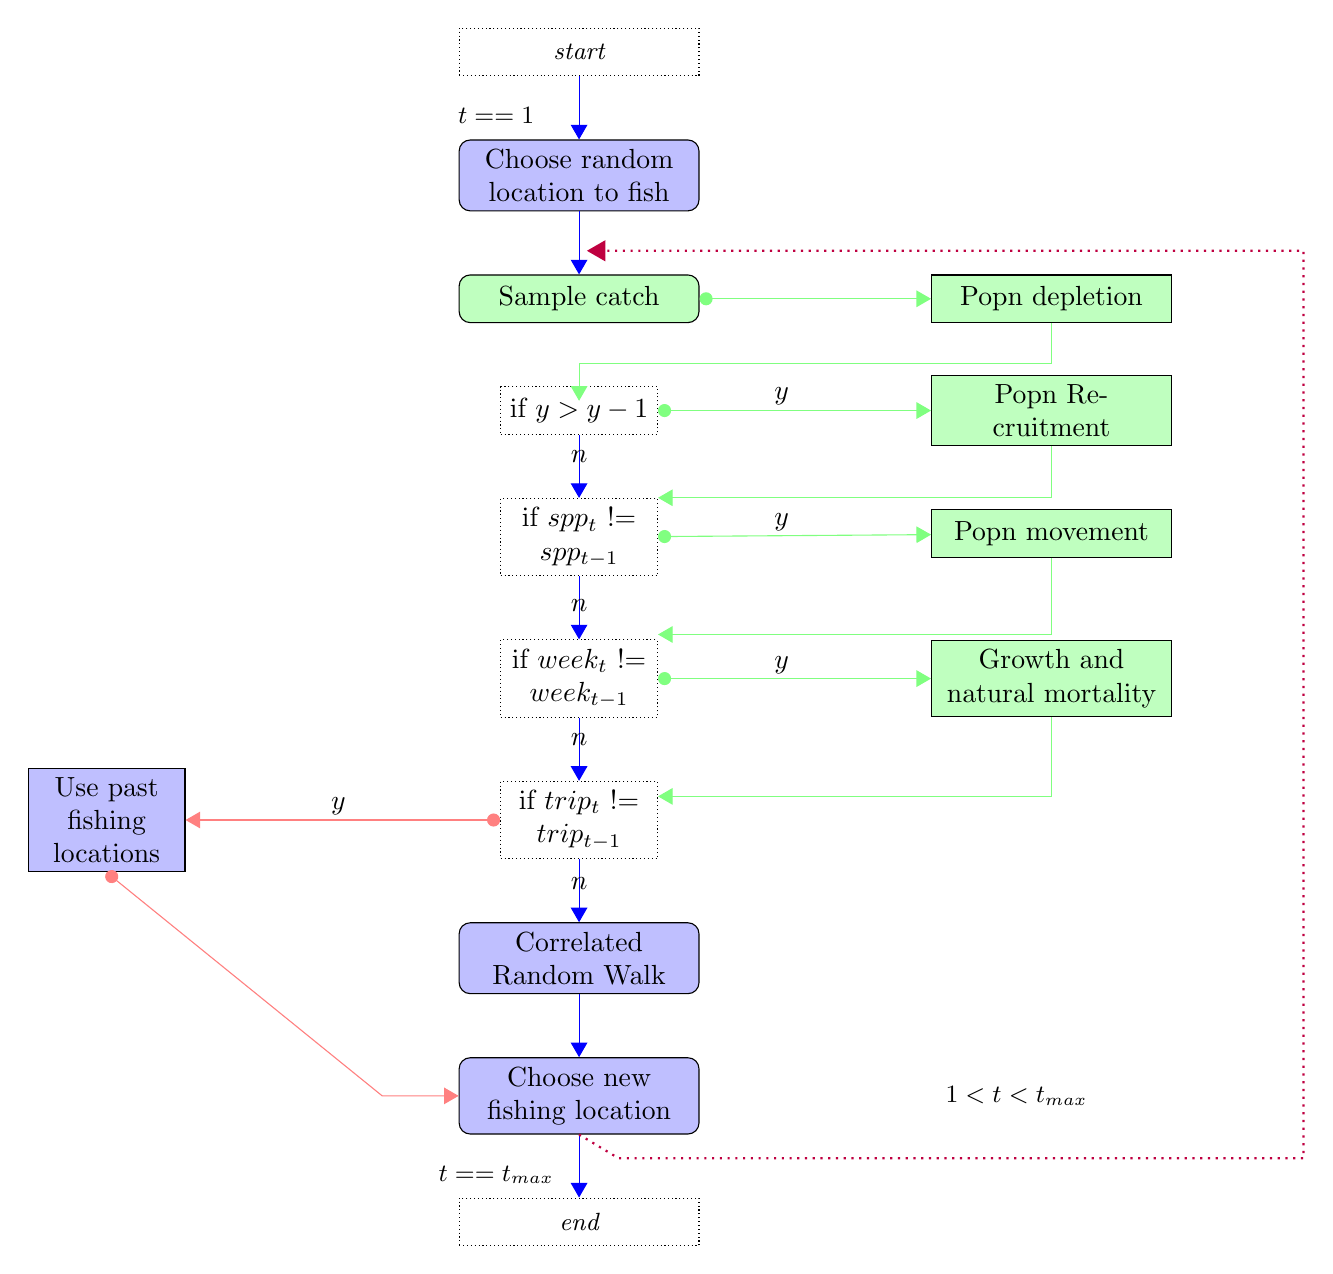
\begin{tikzpicture}[%
    >=triangle 60,              % Nice arrows; your taste may be different
    start chain=going below,    % General flow is top-to-bottom
    node distance=8mm and 60mm, % Global setup of box spacing
    every join/.style={norm}   % Default linetype for connecting boxes
    ]                 
    \label{fig:model}
    % ------------------------------------------------- 
% A few box styles 
% <on chain> *and* <on grid> reduce the need for manual relative
% positioning of nodes
\tikzset{
  base/.style={draw, on chain, on grid, align=center, minimum height=4ex},
  proc/.style={base, rectangle, text width=8em},
  test/.style={base, rectangle, text width=5em},
  term/.style={proc, rounded corners},
  % coord node style is used for placing corners of connecting lines
  coord/.style={coordinate, on chain, on grid, node distance=6mm and 25mm},
  % nmark node style is used for coordinate debugging marks
  nmark/.style={draw, cyan, circle, font={\sffamily\bfseries}},
  % -------------------------------------------------
  % Connector line styles for different parts of the diagram
  norm/.style={->, draw, lcnorm},
  free/.style={->, draw, lcfree},
  cong/.style={->, draw, lccong},
  it/.style={font={\small\itshape}}
}
% -------------------------------------------------
% Start by placing the nodes in the middle
\node [proc, densely dotted, it] (p0) {start};
% Use join to connect a node to the previous one 
\node [term, join, fill=lcnorm!25]      {Choose random location to fish};
\node [term, join, fill=lcfree!25] (p1){Sample catch};
\node [test, densely dotted] (t1) {if $y > y-1$};
\node [test, join, densely dotted] (t2) {if $spp_{t}$ != $spp_{t-1}$};
\node [test, join, densely dotted] (wk) {if $week_{t}$ != $week_{t-1}$};
\node [test, join, densely dotted] (t3) {if $trip_{t}$ != $trip_{t-1}$};
\node [term, join, fill=lcnorm!25]  (p2) {Correlated Random Walk};
\node [term, join, fill=lcnorm!25]  (p3) {Choose new fishing location};
\node [proc, densely dotted, join, it] (p7) {end};

% Right nodes
\node [proc, fill=lcfree!25, right=of p1] (p4) {Popn depletion};
\node [proc, fill=lcfree!25, right=of t1] (p5) {Popn Recruitment};
\node [proc, fill=lcfree!25] (p6) {Popn movement};
\node [proc, fill=lcfree!25, right=of wk] (wk1) {Growth and natural
	mortality};

% left nodes
\node [test, fill=lcnorm!25, left=of t3] (t4) {Use past fishing locations};

% -------------------------------------------------
% A couple of boxes have annotations
\node [below=of p0, it, yshift=1.5em,xshift=-3em] {$t==1$};
\node [right=30mm of p3, it] {$1 < t < t_{max}$};
\node [below=of p3, it,xshift=-3em, yshift=1.5em] {$t == t_{max}$};

% -------------------------------------------------
% First, the straight north-south connections. In each case, we first
% draw a path with a (consistently positioned) annotation node, then
% we draw the arrow itself.
  \draw [*->,lcfree!50] (p1) -- (p4);
\path (t1) to node [near start, xshift=2em, yshift=0.5em] {$y$} (p5); 
  \draw [*->,lcfree!50] (t1) -- (p5);
\path (t2) to node [near start, xshift=2em, yshift=0.5em] {$y$} (p6); 
  \draw [*->,lcfree!50] (t2) -- (p6);
\path (t3) to node [near start, xshift=-3em, yshift=0.5em] {$y$} (t4); 
  \draw [*->,lccong!50] (t3) -- (t4);
\path (wk) to node [near start, xshift=2em, yshift=0.5em] {$y$} (wk1); 
  \draw [*->,lcfree!50] (wk) -- (wk1);

% left to right paths
\path (t1) to node [near start, yshift=-0.2em] {$n$} (t2) ;  
\path (t2) to node [near start, yshift=0.8em] {$n$} (t3) ;  
\path (wk) to node [near start, yshift=-0.2em] {$n$} (t3) ;  
\path (t3) to node [near start, yshift=-0.3em] {$n$} (p2) ;  

% ------------------------------------------------- 
% the twisty connectors. Again, we place the annotation
% first, then draw the connector

\node [coord, left=of p3] (c1)  {};  
\draw [*->,lccong!50] (t4.south) -- (c1) |- (p3);

\node[coord, below=of p4] (c2) {};
\node[coord, above=of t1] (c3) {};
\draw [-<,lcfree!50] (p4.south) -- (c2) |- (c3) |- (t1.north);

\node[coord, below=of p5] (c4) {};
\draw [->,lcfree!50] (p5.south) -- (c4) |- ($(t2.east) + (0,0.5)$);

\node[coord, below=of p6] (c71) {};
\draw [->,lcfree!50] (p6.south) -- (c71) |- ($(wk.east) + (0,0.56)$);

\node[coord, below=of wk1] (c7) {};
\draw [->,lcfree!50] (wk1.south) -- (c7) |- ($(t3.east) + (0,0.3)$);

% -------------------------------------------------
% A last flourish which breaks all the rules
\draw [->,purple, dotted, thick, shorten >=1mm]
  (p3.south) -- ++(5mm,-3mm)  -- ++(87mm,0mm) 
  |- node [black, near end, yshift=1.75em, it]
    {} ($(p1.north) + (0,0.3)$);
% -------------------------------------------------
\end{tikzpicture}
\caption{Overview Schematic of simulation model}
\end{figure}
%%%%%%%%%%%%%%%%%%%%%%%%%%


\subsection{Population dynamics}

The basic population level processes are simulated using a modified two-stage
Deriso-Schnute delay difference model \cite{Deriso1980, Schnute1985}
occurring at the weekly time-step \cite{Dichmont2003}. Here, population
biomass growth and depletion for pre-recruits and fish recruited to the fishery
are modelled separately as a function of previous recruited biomass, intrinsic
population growth and recruitment:

\begin{equation*}
	\begin{split}
	B_{y,w+1} = &\\
	& (1 + \rho) B_{y,w} \cdot e^{-Z_{y,w}} - \rho \cdot e^{-Z_{y,w}} \hspace{2.9cm}
	\times \\  
	& (B_{y,w-1} \cdot e^{-Z_{y,w-1}} + Wt_{R-1} \cdot \alpha_{w-1} \cdot R_{\tilde{y}(y,w-1)})
	\hspace{0.4cm} + \\
	& Wt_{R} \cdot \alpha_{w} \cdot R_{\tilde{y}(y,w)} 
	\end{split}
\end{equation*}

$\rho$ is Brody's coefficient, shown to be approximately equal to $exp(-K)$,
where $K$ is the growth rate from a von bertalanffy logistic growth model
\cite{Schnute1985}.  $Wt_{R-1}$ is the weight of fish prior to recruitment,
while $Wt_{R}$ is the recruited weight.  $\alpha_{w}$ represents the proportion of
fish recruited during the week, while $R_{\tilde{y}}$ is the annual
recruits. \\

Mortality $Z$ can be decomposed to natural mortality, $M$, and fishing
mortality, $F$, where both $M$ and $F$ are instantaneous rates with $M$ fixed
and $F$ calculated by solving the Baranov catch equation \cite{Hilborn1992b}
for $F$:

\begin{equation*}
C_{w} = \frac{F_{w}}{F_{w}+M_{w}} * (1 - e^{-(F_{w} + M_{w})}) * B
\end{equation*}

where $C$ is the summed catch from the fishing model across all fleets and
vessels for the species, year and week respectively, and $B$ the weekly biomass
for the species. \\


\subsection{Recruitment dynamics}

Recruitment is modelled through a function relating the biomass at time of
recruitment to recruits, either as a stochastic Beverton-Holt stock-recruit
form (\cite{Beverton1957}): 

\begin{equation*}
	\begin{split}
	\bar{R} = & \frac{(\alpha * B)}{(\beta + B)} \\
	     R \sim & N[(\bar{R},\sigma^2)]
	\end{split}
\end{equation*}

Where $\alpha$ is the maximum recruitment rate, $\beta$ the spawning stock biomass (SSB)
required to produce half the maximum, and $B$ current SSB; \\

or a stochastic Ricker form \cite{Ricker1954}

\begin{equation*}
	\begin{split}
	\bar{R} = & B * e^{(\alpha - \beta * B)} \\	
   	     R \sim & N[(\bar{R},\sigma^2)]
	\end{split}
\end{equation*}

where $\alpha$ is the maximum productivity per spawner and $\beta$ the density dependent
reduction in productivity as the SSB increases.



\subsection{Population movement}



\subsection{Fleet dynamics}




\section{Theory/calculation}

[A Theory section should extend, not repeat, the background to the article
already dealt with in the Introduction and lay the foundation for further work.
In contrast, a Calculation section represents a practical development from a
theoretical basis.]

HERE DESCRIBE THE PARAMETERISATION, AND ANY COMPARISON AGAINST 'REAL' DATA

\section{Results}

Present simulated closures in terms of \% change in population biomass and
fishery.

[Results should be clear and concise.]

\section{Discussion}

This should explore the significance of the results of the work, not repeat
them. A combined Results
and Discussion section is often appropriate. Avoid extensive citations and
discussion of published
literature.

\section{Conclusions}

The main conclusions of the study may be presented in a short Conclusions
section, which may stand
alone or form a subsection of a Discussion or Results and Discussion section.

\section*{Appendices}

If there is more than one appendix, they should be identified as A, B, etc.
Formulae and equations in appendices should be given separate numbering: Eq.
(A.1), Eq. (A.2), etc.; in a subsequent appendix, Eq. (B.1) and so on.
Similarly for tables and figures: Table A.1; Fig. A.1, etc.

\section*{Abbreviations} Detail any unusual ones used.

\section*{Acknowledgements} those providing help during the research..

\section*{Funding} This work was supported by the MARES doctoral training
program; and the Centre for Environment, Fisheries and Aquaculture Science
seedcorn program.




\section*{References}

\bibliography{simulation_framework}

\end{document}
